% Created by tikzDevice version 0.12.6 on 2025-02-04 18:07:37
% !TEX encoding = UTF-8 Unicode
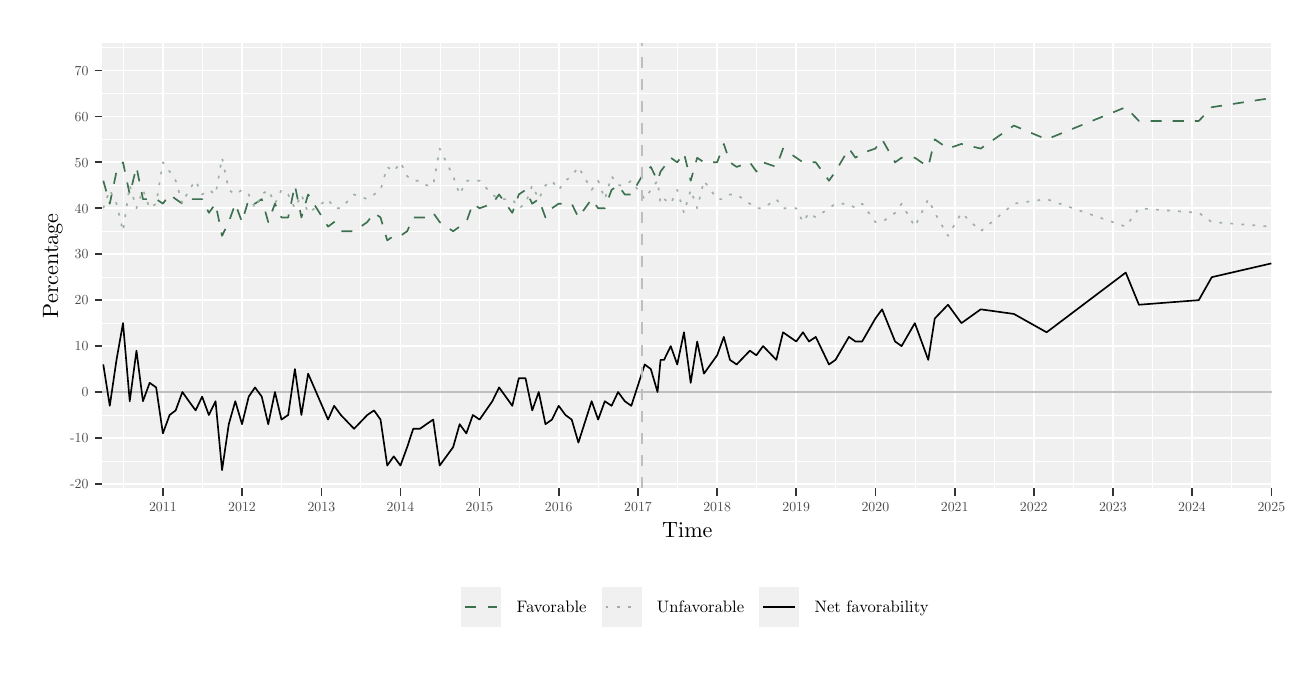
\begin{tikzpicture}[x=1pt,y=1pt]
\definecolor{fillColor}{RGB}{255,255,255}
\path[use as bounding box,fill=fillColor,fill opacity=0.00] (0,0) rectangle (455.30,227.65);
\begin{scope}
\path[clip] (  0.00,  0.00) rectangle (455.30,227.65);
\definecolor{drawColor}{RGB}{255,255,255}
\definecolor{fillColor}{RGB}{255,255,255}

\path[draw=drawColor,line width= 0.6pt,line join=round,line cap=round,fill=fillColor] (  0.00,  0.00) rectangle (455.30,227.65);
\end{scope}
\begin{scope}
\path[clip] ( 26.93, 61.13) rectangle (449.80,222.15);
\definecolor{fillColor}{gray}{0.94}

\path[fill=fillColor] ( 26.93, 61.13) rectangle (449.80,222.15);
\definecolor{drawColor}{RGB}{255,255,255}

\path[draw=drawColor,line width= 0.3pt,line join=round] ( 26.93, 71.09) --
	(449.80, 71.09);

\path[draw=drawColor,line width= 0.3pt,line join=round] ( 26.93, 87.69) --
	(449.80, 87.69);

\path[draw=drawColor,line width= 0.3pt,line join=round] ( 26.93,104.29) --
	(449.80,104.29);

\path[draw=drawColor,line width= 0.3pt,line join=round] ( 26.93,120.89) --
	(449.80,120.89);

\path[draw=drawColor,line width= 0.3pt,line join=round] ( 26.93,137.49) --
	(449.80,137.49);

\path[draw=drawColor,line width= 0.3pt,line join=round] ( 26.93,154.09) --
	(449.80,154.09);

\path[draw=drawColor,line width= 0.3pt,line join=round] ( 26.93,170.69) --
	(449.80,170.69);

\path[draw=drawColor,line width= 0.3pt,line join=round] ( 26.93,187.29) --
	(449.80,187.29);

\path[draw=drawColor,line width= 0.3pt,line join=round] ( 26.93,203.89) --
	(449.80,203.89);

\path[draw=drawColor,line width= 0.3pt,line join=round] ( 26.93,220.49) --
	(449.80,220.49);

\path[draw=drawColor,line width= 0.3pt,line join=round] ( 34.57, 61.13) --
	( 34.57,222.15);

\path[draw=drawColor,line width= 0.3pt,line join=round] ( 63.15, 61.13) --
	( 63.15,222.15);

\path[draw=drawColor,line width= 0.3pt,line join=round] ( 91.78, 61.13) --
	( 91.78,222.15);

\path[draw=drawColor,line width= 0.3pt,line join=round] (120.41, 61.13) --
	(120.41,222.15);

\path[draw=drawColor,line width= 0.3pt,line join=round] (149.00, 61.13) --
	(149.00,222.15);

\path[draw=drawColor,line width= 0.3pt,line join=round] (177.59, 61.13) --
	(177.59,222.15);

\path[draw=drawColor,line width= 0.3pt,line join=round] (206.21, 61.13) --
	(206.21,222.15);

\path[draw=drawColor,line width= 0.3pt,line join=round] (234.84, 61.13) --
	(234.84,222.15);

\path[draw=drawColor,line width= 0.3pt,line join=round] (263.43, 61.13) --
	(263.43,222.15);

\path[draw=drawColor,line width= 0.3pt,line join=round] (292.02, 61.13) --
	(292.02,222.15);

\path[draw=drawColor,line width= 0.3pt,line join=round] (320.64, 61.13) --
	(320.64,222.15);

\path[draw=drawColor,line width= 0.3pt,line join=round] (349.27, 61.13) --
	(349.27,222.15);

\path[draw=drawColor,line width= 0.3pt,line join=round] (377.86, 61.13) --
	(377.86,222.15);

\path[draw=drawColor,line width= 0.3pt,line join=round] (406.45, 61.13) --
	(406.45,222.15);

\path[draw=drawColor,line width= 0.3pt,line join=round] (435.08, 61.13) --
	(435.08,222.15);

\path[draw=drawColor,line width= 0.6pt,line join=round] ( 26.93, 62.79) --
	(449.80, 62.79);

\path[draw=drawColor,line width= 0.6pt,line join=round] ( 26.93, 79.39) --
	(449.80, 79.39);

\path[draw=drawColor,line width= 0.6pt,line join=round] ( 26.93, 95.99) --
	(449.80, 95.99);

\path[draw=drawColor,line width= 0.6pt,line join=round] ( 26.93,112.59) --
	(449.80,112.59);

\path[draw=drawColor,line width= 0.6pt,line join=round] ( 26.93,129.19) --
	(449.80,129.19);

\path[draw=drawColor,line width= 0.6pt,line join=round] ( 26.93,145.79) --
	(449.80,145.79);

\path[draw=drawColor,line width= 0.6pt,line join=round] ( 26.93,162.39) --
	(449.80,162.39);

\path[draw=drawColor,line width= 0.6pt,line join=round] ( 26.93,178.99) --
	(449.80,178.99);

\path[draw=drawColor,line width= 0.6pt,line join=round] ( 26.93,195.59) --
	(449.80,195.59);

\path[draw=drawColor,line width= 0.6pt,line join=round] ( 26.93,212.19) --
	(449.80,212.19);

\path[draw=drawColor,line width= 0.6pt,line join=round] ( 48.86, 61.13) --
	( 48.86,222.15);

\path[draw=drawColor,line width= 0.6pt,line join=round] ( 77.45, 61.13) --
	( 77.45,222.15);

\path[draw=drawColor,line width= 0.6pt,line join=round] (106.12, 61.13) --
	(106.12,222.15);

\path[draw=drawColor,line width= 0.6pt,line join=round] (134.70, 61.13) --
	(134.70,222.15);

\path[draw=drawColor,line width= 0.6pt,line join=round] (163.29, 61.13) --
	(163.29,222.15);

\path[draw=drawColor,line width= 0.6pt,line join=round] (191.88, 61.13) --
	(191.88,222.15);

\path[draw=drawColor,line width= 0.6pt,line join=round] (220.55, 61.13) --
	(220.55,222.15);

\path[draw=drawColor,line width= 0.6pt,line join=round] (249.14, 61.13) --
	(249.14,222.15);

\path[draw=drawColor,line width= 0.6pt,line join=round] (277.72, 61.13) --
	(277.72,222.15);

\path[draw=drawColor,line width= 0.6pt,line join=round] (306.31, 61.13) --
	(306.31,222.15);

\path[draw=drawColor,line width= 0.6pt,line join=round] (334.98, 61.13) --
	(334.98,222.15);

\path[draw=drawColor,line width= 0.6pt,line join=round] (363.57, 61.13) --
	(363.57,222.15);

\path[draw=drawColor,line width= 0.6pt,line join=round] (392.15, 61.13) --
	(392.15,222.15);

\path[draw=drawColor,line width= 0.6pt,line join=round] (420.74, 61.13) --
	(420.74,222.15);

\path[draw=drawColor,line width= 0.6pt,line join=round] (449.41, 61.13) --
	(449.41,222.15);
\definecolor{drawColor}{RGB}{190,190,190}

\path[draw=drawColor,line width= 0.6pt,line join=round] ( 26.93, 95.99) -- (449.80, 95.99);
\definecolor{drawColor}{RGB}{60,113,79}

\path[draw=drawColor,line width= 0.6pt,dash pattern=on 4pt off 4pt ,line join=round] ( 27.32,172.35) --
	( 29.67,164.05) --
	( 32.10,175.67) --
	( 34.45,178.99) --
	( 36.88,167.37) --
	( 39.31,177.33) --
	( 41.65,165.71) --
	( 44.08,165.71) --
	( 46.43,165.71) --
	( 48.86,164.05) --
	( 51.29,167.37) --
	( 53.48,165.71) --
	( 55.91,164.05) --
	( 58.26,165.71) --
	( 60.69,165.71) --
	( 63.04,165.71) --
	( 65.47,160.73) --
	( 67.89,164.05) --
	( 70.24,152.43) --
	( 72.67,157.41) --
	( 75.02,164.05) --
	( 77.45,157.41) --
	( 79.88,165.71) --
	( 82.15,164.05) --
	( 84.58,165.71) --
	( 86.93,157.41) --
	( 89.35,164.05) --
	( 91.70,159.07) --
	( 94.13,159.07) --
	( 96.56,170.69) --
	( 98.91,159.07) --
	(101.34,167.37) --
	(108.54,155.75) --
	(110.74,157.41) --
	(113.16,154.09) --
	(117.94,154.09) --
	(122.72,157.41) --
	(125.15,160.73) --
	(127.50,159.07) --
	(129.93,150.77) --
	(132.28,152.43) --
	(134.70,152.43) --
	(137.13,154.09) --
	(139.32,159.07) --
	(141.75,159.07) --
	(144.10,159.07) --
	(146.53,160.73) --
	(148.88,157.41) --
	(153.74,154.09) --
	(156.09,155.75) --
	(158.51,157.41) --
	(160.86,164.05) --
	(163.29,162.39) --
	(167.91,164.05) --
	(170.34,167.37) --
	(175.12,160.73) --
	(177.47,167.37) --
	(179.90,169.03) --
	(182.32,164.05) --
	(184.67,165.71) --
	(187.10,159.07) --
	(189.45,162.39) --
	(191.88,164.05) --
	(194.31,164.05) --
	(196.58,164.05) --
	(199.01,159.07) --
	(203.79,165.71) --
	(206.14,162.39) --
	(208.56,162.39) --
	(210.99,169.03) --
	(213.34,170.69) --
	(215.77,167.37) --
	(218.12,167.37) --
	(222.97,175.67) --
	(225.17,177.33) --
	(227.60,172.35) --
	(228.69,175.67) --
	(229.95,177.33) --
	(232.37,180.65) --
	(234.72,178.99) --
	(237.15,182.31) --
	(239.58,172.35) --
	(241.93,180.65) --
	(244.36,178.99) --
	(249.14,178.99) --
	(251.56,185.63) --
	(253.76,178.99) --
	(256.18,177.33) --
	(260.96,178.99) --
	(263.31,175.67) --
	(265.74,178.99) --
	(270.52,177.33) --
	(272.95,183.97) --
	(277.72,180.65) --
	(280.15,178.99) --
	(282.34,178.99) --
	(284.77,178.99) --
	(289.55,172.35) --
	(291.90,175.67) --
	(296.76,183.97) --
	(299.11,180.65) --
	(301.53,182.31) --
	(306.31,183.97) --
	(308.74,187.29) --
	(313.44,178.99) --
	(315.79,180.65) --
	(320.57,180.65) --
	(325.42,177.33) --
	(327.77,187.29) --
	(332.55,183.97) --
	(337.41,185.63) --
	(344.38,183.97) --
	(356.36,192.27) --
	(368.19,187.29) --
	(396.78,198.91) --
	(401.55,193.93) --
	(423.17,193.93) --
	(427.87,198.91) --
	(449.41,202.23);
\definecolor{drawColor}{RGB}{157,176,162}

\path[draw=drawColor,line width= 0.6pt,dash pattern=on 1pt off 3pt ,line join=round] ( 27.32,162.39) --
	( 29.67,169.03) --
	( 32.10,164.05) --
	( 34.45,154.09) --
	( 36.88,170.69) --
	( 39.31,162.39) --
	( 41.65,169.03) --
	( 44.08,162.39) --
	( 46.43,164.05) --
	( 48.86,178.99) --
	( 51.29,175.67) --
	( 53.48,172.35) --
	( 55.91,164.05) --
	( 58.26,169.03) --
	( 60.69,172.35) --
	( 63.04,167.37) --
	( 65.47,169.03) --
	( 67.89,167.37) --
	( 70.24,180.65) --
	( 72.67,169.03) --
	( 75.02,167.37) --
	( 77.45,169.03) --
	( 79.88,167.37) --
	( 82.15,162.39) --
	( 84.58,167.37) --
	( 86.93,169.03) --
	( 89.35,164.05) --
	( 91.70,169.03) --
	( 94.13,167.37) --
	( 96.56,162.39) --
	( 98.91,167.37) --
	(101.34,160.73) --
	(108.54,165.71) --
	(110.74,162.39) --
	(113.16,162.39) --
	(117.94,167.37) --
	(122.72,165.71) --
	(125.15,167.37) --
	(127.50,169.03) --
	(129.93,177.33) --
	(132.28,175.67) --
	(134.70,178.99) --
	(137.13,174.01) --
	(139.32,172.35) --
	(141.75,172.35) --
	(144.10,170.69) --
	(146.53,170.69) --
	(148.88,183.97) --
	(153.74,174.01) --
	(156.09,167.37) --
	(158.51,172.35) --
	(160.86,172.35) --
	(163.29,172.35) --
	(167.91,167.37) --
	(170.34,165.71) --
	(175.12,165.71) --
	(177.47,162.39) --
	(179.90,164.05) --
	(182.32,170.69) --
	(184.67,165.71) --
	(187.10,170.69) --
	(189.45,172.35) --
	(191.88,169.03) --
	(194.31,172.35) --
	(196.58,174.01) --
	(199.01,177.33) --
	(203.79,169.03) --
	(206.14,172.35) --
	(208.56,165.71) --
	(210.99,174.01) --
	(213.34,170.69) --
	(215.77,170.69) --
	(218.12,172.35) --
	(222.97,165.71) --
	(225.17,169.03) --
	(227.60,172.35) --
	(228.69,164.05) --
	(229.95,165.71) --
	(232.37,164.05) --
	(234.72,169.03) --
	(237.15,160.73) --
	(239.58,169.03) --
	(241.93,162.39) --
	(244.36,172.35) --
	(249.14,165.71) --
	(251.56,165.71) --
	(253.76,167.37) --
	(256.18,167.37) --
	(260.96,164.05) --
	(263.31,162.39) --
	(265.74,162.39) --
	(270.52,165.71) --
	(272.95,162.39) --
	(277.72,162.39) --
	(280.15,157.41) --
	(282.34,160.73) --
	(284.77,159.07) --
	(289.55,162.39) --
	(291.90,164.05) --
	(296.76,164.05) --
	(299.11,162.39) --
	(301.53,164.05) --
	(306.31,157.41) --
	(308.74,157.41) --
	(313.44,160.73) --
	(315.79,164.05) --
	(320.57,155.75) --
	(325.42,165.71) --
	(327.77,160.73) --
	(332.55,152.43) --
	(337.41,160.73) --
	(344.38,154.09) --
	(356.36,164.05) --
	(368.19,165.71) --
	(396.78,155.75) --
	(401.55,162.39) --
	(423.17,160.73) --
	(427.87,157.41) --
	(449.41,155.75);
\definecolor{drawColor}{RGB}{0,0,0}

\path[draw=drawColor,line width= 0.6pt,line join=round] ( 27.32,105.95) --
	( 29.67, 91.01) --
	( 32.10,107.61) --
	( 34.45,120.89) --
	( 36.88, 92.67) --
	( 39.31,110.93) --
	( 41.65, 92.67) --
	( 44.08, 99.31) --
	( 46.43, 97.65) --
	( 48.86, 81.05) --
	( 51.29, 87.69) --
	( 53.48, 89.35) --
	( 55.91, 95.99) --
	( 58.26, 92.67) --
	( 60.69, 89.35) --
	( 63.04, 94.33) --
	( 65.47, 87.69) --
	( 67.89, 92.67) --
	( 70.24, 67.77) --
	( 72.67, 84.37) --
	( 75.02, 92.67) --
	( 77.45, 84.37) --
	( 79.88, 94.33) --
	( 82.15, 97.65) --
	( 84.58, 94.33) --
	( 86.93, 84.37) --
	( 89.35, 95.99) --
	( 91.70, 86.03) --
	( 94.13, 87.69) --
	( 96.56,104.29) --
	( 98.91, 87.69) --
	(101.34,102.63) --
	(108.54, 86.03) --
	(110.74, 91.01) --
	(113.16, 87.69) --
	(117.94, 82.71) --
	(122.72, 87.69) --
	(125.15, 89.35) --
	(127.50, 86.03) --
	(129.93, 69.43) --
	(132.28, 72.75) --
	(134.70, 69.43) --
	(137.13, 76.07) --
	(139.32, 82.71) --
	(141.75, 82.71) --
	(144.10, 84.37) --
	(146.53, 86.03) --
	(148.88, 69.43) --
	(153.74, 76.07) --
	(156.09, 84.37) --
	(158.51, 81.05) --
	(160.86, 87.69) --
	(163.29, 86.03) --
	(167.91, 92.67) --
	(170.34, 97.65) --
	(175.12, 91.01) --
	(177.47,100.97) --
	(179.90,100.97) --
	(182.32, 89.35) --
	(184.67, 95.99) --
	(187.10, 84.37) --
	(189.45, 86.03) --
	(191.88, 91.01) --
	(194.31, 87.69) --
	(196.58, 86.03) --
	(199.01, 77.73) --
	(203.79, 92.67) --
	(206.14, 86.03) --
	(208.56, 92.67) --
	(210.99, 91.01) --
	(213.34, 95.99) --
	(215.77, 92.67) --
	(218.12, 91.01) --
	(222.97,105.95) --
	(225.17,104.29) --
	(227.60, 95.99) --
	(228.69,107.61) --
	(229.95,107.61) --
	(232.37,112.59) --
	(234.72,105.95) --
	(237.15,117.57) --
	(239.58, 99.31) --
	(241.93,114.25) --
	(244.36,102.63) --
	(249.14,109.27) --
	(251.56,115.91) --
	(253.76,107.61) --
	(256.18,105.95) --
	(260.96,110.93) --
	(263.31,109.27) --
	(265.74,112.59) --
	(270.52,107.61) --
	(272.95,117.57) --
	(277.72,114.25) --
	(280.15,117.57) --
	(282.34,114.25) --
	(284.77,115.91) --
	(289.55,105.95) --
	(291.90,107.61) --
	(296.76,115.91) --
	(299.11,114.25) --
	(301.53,114.25) --
	(306.31,122.55) --
	(308.74,125.87) --
	(313.44,114.25) --
	(315.79,112.59) --
	(320.57,120.89) --
	(325.42,107.61) --
	(327.77,122.55) --
	(332.55,127.53) --
	(337.41,120.89) --
	(344.38,125.87) --
	(356.36,124.21) --
	(368.19,117.57) --
	(396.78,139.15) --
	(401.55,127.53) --
	(423.17,129.19) --
	(427.87,137.49) --
	(449.41,142.47);
\definecolor{drawColor}{RGB}{190,190,190}

\path[draw=drawColor,line width= 0.6pt,dash pattern=on 4pt off 4pt ,line join=round] (222.03, 61.13) -- (222.03,222.15);
\end{scope}
\begin{scope}
\path[clip] (  0.00,  0.00) rectangle (455.30,227.65);
\definecolor{drawColor}{gray}{0.30}

\node[text=drawColor,anchor=base east,inner sep=0pt, outer sep=0pt, scale=  0.50] at ( 21.98, 61.07) {-20};

\node[text=drawColor,anchor=base east,inner sep=0pt, outer sep=0pt, scale=  0.50] at ( 21.98, 77.67) {-10};

\node[text=drawColor,anchor=base east,inner sep=0pt, outer sep=0pt, scale=  0.50] at ( 21.98, 94.27) {0};

\node[text=drawColor,anchor=base east,inner sep=0pt, outer sep=0pt, scale=  0.50] at ( 21.98,110.87) {10};

\node[text=drawColor,anchor=base east,inner sep=0pt, outer sep=0pt, scale=  0.50] at ( 21.98,127.47) {20};

\node[text=drawColor,anchor=base east,inner sep=0pt, outer sep=0pt, scale=  0.50] at ( 21.98,144.07) {30};

\node[text=drawColor,anchor=base east,inner sep=0pt, outer sep=0pt, scale=  0.50] at ( 21.98,160.67) {40};

\node[text=drawColor,anchor=base east,inner sep=0pt, outer sep=0pt, scale=  0.50] at ( 21.98,177.27) {50};

\node[text=drawColor,anchor=base east,inner sep=0pt, outer sep=0pt, scale=  0.50] at ( 21.98,193.87) {60};

\node[text=drawColor,anchor=base east,inner sep=0pt, outer sep=0pt, scale=  0.50] at ( 21.98,210.47) {70};
\end{scope}
\begin{scope}
\path[clip] (  0.00,  0.00) rectangle (455.30,227.65);
\definecolor{drawColor}{gray}{0.20}

\path[draw=drawColor,line width= 0.6pt,line join=round] ( 24.18, 62.79) --
	( 26.93, 62.79);

\path[draw=drawColor,line width= 0.6pt,line join=round] ( 24.18, 79.39) --
	( 26.93, 79.39);

\path[draw=drawColor,line width= 0.6pt,line join=round] ( 24.18, 95.99) --
	( 26.93, 95.99);

\path[draw=drawColor,line width= 0.6pt,line join=round] ( 24.18,112.59) --
	( 26.93,112.59);

\path[draw=drawColor,line width= 0.6pt,line join=round] ( 24.18,129.19) --
	( 26.93,129.19);

\path[draw=drawColor,line width= 0.6pt,line join=round] ( 24.18,145.79) --
	( 26.93,145.79);

\path[draw=drawColor,line width= 0.6pt,line join=round] ( 24.18,162.39) --
	( 26.93,162.39);

\path[draw=drawColor,line width= 0.6pt,line join=round] ( 24.18,178.99) --
	( 26.93,178.99);

\path[draw=drawColor,line width= 0.6pt,line join=round] ( 24.18,195.59) --
	( 26.93,195.59);

\path[draw=drawColor,line width= 0.6pt,line join=round] ( 24.18,212.19) --
	( 26.93,212.19);
\end{scope}
\begin{scope}
\path[clip] (  0.00,  0.00) rectangle (455.30,227.65);
\definecolor{drawColor}{gray}{0.20}

\path[draw=drawColor,line width= 0.6pt,line join=round] ( 48.86, 58.38) --
	( 48.86, 61.13);

\path[draw=drawColor,line width= 0.6pt,line join=round] ( 77.45, 58.38) --
	( 77.45, 61.13);

\path[draw=drawColor,line width= 0.6pt,line join=round] (106.12, 58.38) --
	(106.12, 61.13);

\path[draw=drawColor,line width= 0.6pt,line join=round] (134.70, 58.38) --
	(134.70, 61.13);

\path[draw=drawColor,line width= 0.6pt,line join=round] (163.29, 58.38) --
	(163.29, 61.13);

\path[draw=drawColor,line width= 0.6pt,line join=round] (191.88, 58.38) --
	(191.88, 61.13);

\path[draw=drawColor,line width= 0.6pt,line join=round] (220.55, 58.38) --
	(220.55, 61.13);

\path[draw=drawColor,line width= 0.6pt,line join=round] (249.14, 58.38) --
	(249.14, 61.13);

\path[draw=drawColor,line width= 0.6pt,line join=round] (277.72, 58.38) --
	(277.72, 61.13);

\path[draw=drawColor,line width= 0.6pt,line join=round] (306.31, 58.38) --
	(306.31, 61.13);

\path[draw=drawColor,line width= 0.6pt,line join=round] (334.98, 58.38) --
	(334.98, 61.13);

\path[draw=drawColor,line width= 0.6pt,line join=round] (363.57, 58.38) --
	(363.57, 61.13);

\path[draw=drawColor,line width= 0.6pt,line join=round] (392.15, 58.38) --
	(392.15, 61.13);

\path[draw=drawColor,line width= 0.6pt,line join=round] (420.74, 58.38) --
	(420.74, 61.13);

\path[draw=drawColor,line width= 0.6pt,line join=round] (449.41, 58.38) --
	(449.41, 61.13);
\end{scope}
\begin{scope}
\path[clip] (  0.00,  0.00) rectangle (455.30,227.65);
\definecolor{drawColor}{gray}{0.30}

\node[text=drawColor,anchor=base,inner sep=0pt, outer sep=0pt, scale=  0.50] at ( 48.86, 52.74) {2011};

\node[text=drawColor,anchor=base,inner sep=0pt, outer sep=0pt, scale=  0.50] at ( 77.45, 52.74) {2012};

\node[text=drawColor,anchor=base,inner sep=0pt, outer sep=0pt, scale=  0.50] at (106.12, 52.74) {2013};

\node[text=drawColor,anchor=base,inner sep=0pt, outer sep=0pt, scale=  0.50] at (134.70, 52.74) {2014};

\node[text=drawColor,anchor=base,inner sep=0pt, outer sep=0pt, scale=  0.50] at (163.29, 52.74) {2015};

\node[text=drawColor,anchor=base,inner sep=0pt, outer sep=0pt, scale=  0.50] at (191.88, 52.74) {2016};

\node[text=drawColor,anchor=base,inner sep=0pt, outer sep=0pt, scale=  0.50] at (220.55, 52.74) {2017};

\node[text=drawColor,anchor=base,inner sep=0pt, outer sep=0pt, scale=  0.50] at (249.14, 52.74) {2018};

\node[text=drawColor,anchor=base,inner sep=0pt, outer sep=0pt, scale=  0.50] at (277.72, 52.74) {2019};

\node[text=drawColor,anchor=base,inner sep=0pt, outer sep=0pt, scale=  0.50] at (306.31, 52.74) {2020};

\node[text=drawColor,anchor=base,inner sep=0pt, outer sep=0pt, scale=  0.50] at (334.98, 52.74) {2021};

\node[text=drawColor,anchor=base,inner sep=0pt, outer sep=0pt, scale=  0.50] at (363.57, 52.74) {2022};

\node[text=drawColor,anchor=base,inner sep=0pt, outer sep=0pt, scale=  0.50] at (392.15, 52.74) {2023};

\node[text=drawColor,anchor=base,inner sep=0pt, outer sep=0pt, scale=  0.50] at (420.74, 52.74) {2024};

\node[text=drawColor,anchor=base,inner sep=0pt, outer sep=0pt, scale=  0.50] at (449.41, 52.74) {2025};
\end{scope}
\begin{scope}
\path[clip] (  0.00,  0.00) rectangle (455.30,227.65);
\definecolor{drawColor}{RGB}{0,0,0}

\node[text=drawColor,anchor=base,inner sep=0pt, outer sep=0pt, scale=  0.80] at (238.37, 43.51) {Time};
\end{scope}
\begin{scope}
\path[clip] (  0.00,  0.00) rectangle (455.30,227.65);
\definecolor{drawColor}{RGB}{0,0,0}

\node[text=drawColor,rotate= 90.00,anchor=base,inner sep=0pt, outer sep=0pt, scale=  0.80] at ( 11.01,141.64) {Percentage};
\end{scope}
\begin{scope}
\path[clip] (  0.00,  0.00) rectangle (455.30,227.65);
\definecolor{fillColor}{RGB}{255,255,255}

\path[fill=fillColor] (145.71,  5.50) rectangle (331.02, 30.95);
\end{scope}
\begin{scope}
\path[clip] (  0.00,  0.00) rectangle (455.30,227.65);
\definecolor{fillColor}{gray}{0.94}

\path[fill=fillColor] (156.71, 11.00) rectangle (171.17, 25.45);
\end{scope}
\begin{scope}
\path[clip] (  0.00,  0.00) rectangle (455.30,227.65);
\definecolor{drawColor}{RGB}{60,113,79}

\path[draw=drawColor,line width= 0.6pt,dash pattern=on 4pt off 4pt ,line join=round] (158.16, 18.23) -- (169.72, 18.23);
\end{scope}
\begin{scope}
\path[clip] (  0.00,  0.00) rectangle (455.30,227.65);
\definecolor{fillColor}{gray}{0.94}

\path[fill=fillColor] (207.43, 11.00) rectangle (221.88, 25.45);
\end{scope}
\begin{scope}
\path[clip] (  0.00,  0.00) rectangle (455.30,227.65);
\definecolor{drawColor}{RGB}{157,176,162}

\path[draw=drawColor,line width= 0.6pt,dash pattern=on 1pt off 3pt ,line join=round] (208.87, 18.23) -- (220.44, 18.23);
\end{scope}
\begin{scope}
\path[clip] (  0.00,  0.00) rectangle (455.30,227.65);
\definecolor{fillColor}{gray}{0.94}

\path[fill=fillColor] (264.39, 11.00) rectangle (278.84, 25.45);
\end{scope}
\begin{scope}
\path[clip] (  0.00,  0.00) rectangle (455.30,227.65);
\definecolor{drawColor}{RGB}{0,0,0}

\path[draw=drawColor,line width= 0.6pt,line join=round] (265.84, 18.23) -- (277.40, 18.23);
\end{scope}
\begin{scope}
\path[clip] (  0.00,  0.00) rectangle (455.30,227.65);
\definecolor{drawColor}{RGB}{0,0,0}

\node[text=drawColor,anchor=base west,inner sep=0pt, outer sep=0pt, scale=  0.60] at (176.67, 16.16) {Favorable};
\end{scope}
\begin{scope}
\path[clip] (  0.00,  0.00) rectangle (455.30,227.65);
\definecolor{drawColor}{RGB}{0,0,0}

\node[text=drawColor,anchor=base west,inner sep=0pt, outer sep=0pt, scale=  0.60] at (227.38, 16.16) {Unfavorable};
\end{scope}
\begin{scope}
\path[clip] (  0.00,  0.00) rectangle (455.30,227.65);
\definecolor{drawColor}{RGB}{0,0,0}

\node[text=drawColor,anchor=base west,inner sep=0pt, outer sep=0pt, scale=  0.60] at (284.34, 16.16) {Net favorability};
\end{scope}
\end{tikzpicture}
